\section{Explicación Esquemática de acados}

\subsection{¿Qué problema resuelve acados?}

acados resuelve el problema fundamental del control predictivo:

\begin{center}
\fbox{
\begin{minipage}{0.85\textwidth}
\textbf{Pregunta del control:} \\
``Dado el estado actual de mi sistema, ¿qué controles debo aplicar \underline{ahora} y en el futuro cercano para lograr mi objetivo de manera óptima?''
\end{minipage}
}
\end{center}

\subsection{Diagrama del Proceso Completo}

\begin{figure}[h]
\centering
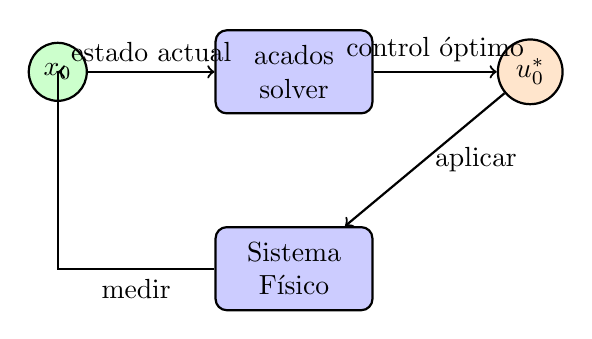
\begin{tikzpicture}[node distance=2cm, auto, thick,
    block/.style={rectangle, draw, fill=blue!20, text width=5em, text centered, rounded corners, minimum height=3em},
    input/.style={circle, draw, fill=green!20, text centered, minimum size=2em},
    output/.style={circle, draw, fill=orange!20, text centered, minimum size=2em}]

% Nodes
\node [input] (state) {$x_0$};
\node [block, right of=state, node distance=3cm] (acados) {acados \\ solver};
\node [output, right of=acados, node distance=3cm] (control) {$u_0^*$};
\node [block, below of=acados, node distance=2.5cm] (system) {Sistema \\ Físico};

% Arrows
\draw[->] (state) -- node[above] {estado actual} (acados);
\draw[->] (acados) -- node[above] {control óptimo} (control);
\draw[->] (control) -- node[right] {aplicar} (system);
\draw[->] (system) -| node[below, near start] {medir} ++(-3,0) |- (state);

\end{tikzpicture}
\caption{Ciclo de control con acados}
\end{figure}

\subsection{¿Cómo lo hace? - Los 5 Pasos Principales}

\begin{enumerate}
\item \textbf{MODELAR} el sistema (ecuaciones dinámicas)
\item \textbf{DEFINIR} el objetivo (función de costo)
\item \textbf{ESTABLECER} restricciones (límites físicos)
\item \textbf{RESOLVER} el problema de optimización
\item \textbf{APLICAR} el primer control y repetir
\end{enumerate}

\subsubsection{Paso 1: Modelar el Sistema}

\begin{center}
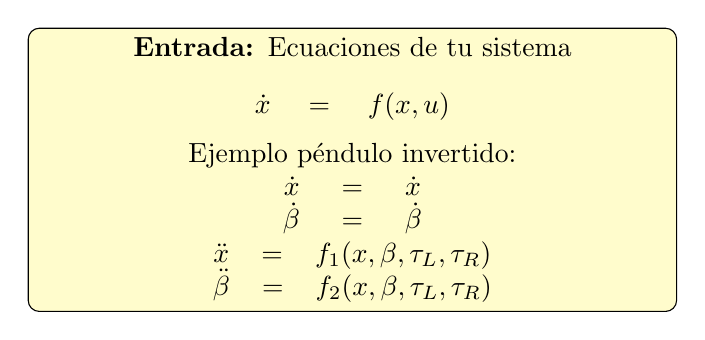
\begin{tikzpicture}
\node[draw, rounded corners, fill=yellow!20, text width=8cm, align=center] {
\textbf{Entrada:} Ecuaciones de tu sistema \\[0.3cm]
$\dot{x} = f(x, u)$ \\[0.2cm]
Ejemplo péndulo invertido: \\
$\dot{x} = \dot{x}$ \\
$\dot{\beta} = \dot{\beta}$ \\
$\ddot{x} = f_1(x, \beta, \tau_L, \tau_R)$ \\
$\ddot{\beta} = f_2(x, \beta, \tau_L, \tau_R)$
};
\end{tikzpicture}
\end{center}

\textbf{En código:}
\begin{verbatim}
model.x = [x; beta; x_dot; beta_dot];  % Estados
model.u = [tau_L; tau_R];               % Controles
model.f_expl_expr = [x_dot; beta_dot; x_ddot; beta_ddot];
\end{verbatim}

\subsubsection{Paso 2: Definir el Objetivo}

\begin{center}
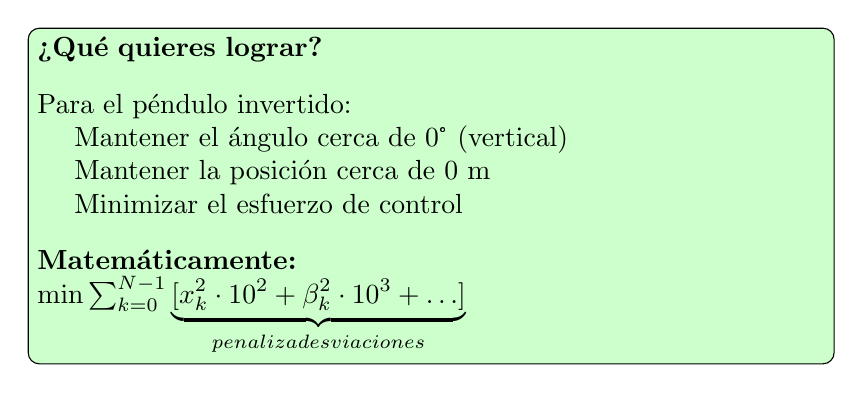
\begin{tikzpicture}
\node[draw, rounded corners, fill=green!20, text width=10cm, align=left] {
\textbf{¿Qué quieres lograr?} \\[0.3cm]
Para el péndulo invertido: \\
\quad $\checkmark$ Mantener el ángulo cerca de 0° (vertical) \\
\quad $\checkmark$ Mantener la posición cerca de 0 m \\
\quad $\checkmark$ Minimizar el esfuerzo de control \\[0.3cm]
\textbf{Matemáticamente:} \\
$\min \sum_{k=0}^{N-1} \underbrace{[x_k^2 \cdot 10^2 + \beta_k^2 \cdot 10^3 + \ldots]}_{\text{penaliza desviaciones}}$
};
\end{tikzpicture}
\end{center}

\textbf{En código:}
\begin{verbatim}
W_x = diag([1e2, 1e3, 1e2, 1e3]);  % Pesos: posición, ángulo, velocidades
W_u = 1e-1 * eye(2);                % Peso del control
ocp.cost.W = blkdiag(W_x, W_u);
\end{verbatim}

\subsubsection{Paso 3: Establecer Restricciones}

\begin{center}
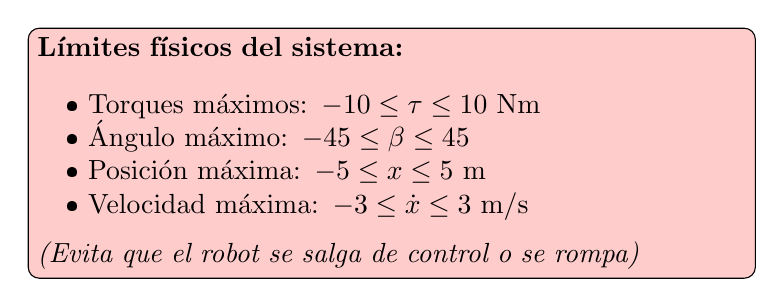
\begin{tikzpicture}
\node[draw, rounded corners, fill=red!20, text width=9cm, align=left] {
\textbf{Límites físicos del sistema:} \\[0.3cm]
\quad • Torques máximos: $-10 \leq \tau \leq 10$ Nm \\
\quad • Ángulo máximo: $-45° \leq \beta \leq 45°$ \\
\quad • Posición máxima: $-5 \leq x \leq 5$ m \\
\quad • Velocidad máxima: $-3 \leq \dot{x} \leq 3$ m/s \\[0.2cm]
\textit{(Evita que el robot se salga de control o se rompa)}
};
\end{tikzpicture}
\end{center}

\textbf{En código:}
\begin{verbatim}
ocp.constraints.lbu = [-10; -10];   % Límite inferior control
ocp.constraints.ubu = [10; 10];     % Límite superior control
ocp.constraints.lbx = [-5; -pi/4; -3; -pi];  % Límites estados
ocp.constraints.ubx = [5; pi/4; 3; pi];
\end{verbatim}

\subsubsection{Paso 4: Resolver el Problema}



Esto es lo que hace acados internamente:

\begin{enumerate}
\item \textbf{Discretiza el tiempo}: Divide el horizonte de 1 segundo en $N=40$ pasos
\item \textbf{Linealiza}: Aproxima tu sistema no lineal localmente con líneas rectas
\item \textbf{Resuelve QP}: Usa álgebra lineal ultra-rápida (BLASFEO + HPIPM)
\item \textbf{Itera}: Mejora la solución (método SQP)
\end{enumerate}

\subsection{Diagrama Temporal del NMPC}

\begin{figure}[h]
\centering
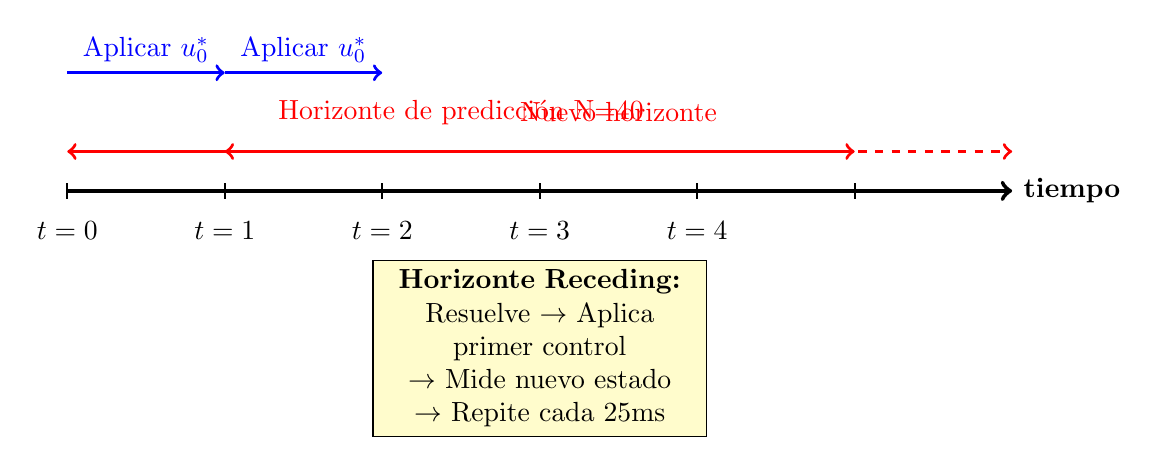
\begin{tikzpicture}
% Time axis
\draw[->, ultra thick] (0,0) -- (12,0) node[right] {\textbf{tiempo}};

% Time steps
\foreach \x in {0,2,4,6,8,10} {
    \draw[thick] (\x, -0.1) -- (\x, 0.1);
}
\node at (0,-0.5) {$t=0$};
\node at (2,-0.5) {$t=1$};
\node at (4,-0.5) {$t=2$};
\node at (6,-0.5) {$t=3$};
\node at (8,-0.5) {$t=4$};

% First prediction horizon
\draw[<->, red, very thick] (0,0.5) -- (10,0.5);
\node[red] at (5,1) {Horizonte de predicción N=40};

% Apply first control
\draw[->, blue, very thick] (0,1.5) -- (2,1.5);
\node[blue, above] at (1,1.5) {Aplicar $u_0^*$};

% Second prediction horizon (shifted)
\draw[<->, red, very thick, dashed] (2,0.5) -- (12,0.5);
\node[red] at (7,1) {Nuevo horizonte};

% Apply second control
\draw[->, blue, very thick] (2,1.5) -- (4,1.5);
\node[blue, above] at (3,1.5) {Aplicar $u_0^*$};

\node[draw, fill=yellow!20, text width=4cm, align=center] at (6,-2) {
\textbf{Horizonte Receding:} \\
Resuelve $\rightarrow$ Aplica primer control \\
$\rightarrow$ Mide nuevo estado \\
$\rightarrow$ Repite cada 25ms
};

\end{tikzpicture}
\caption{Principio del horizonte deslizante (receding horizon)}
\end{figure}

\subsection{Arquitectura Modular de acados}

\begin{figure}[h]
\centering
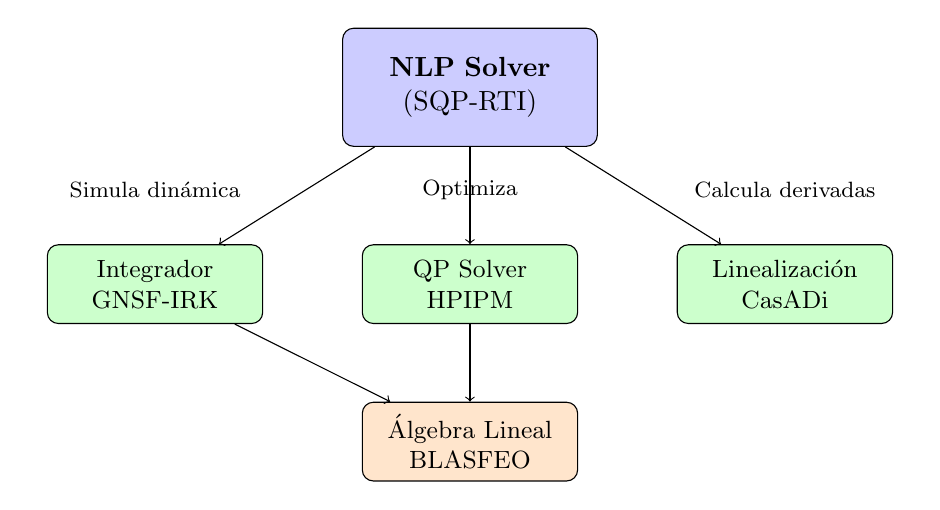
\begin{tikzpicture}[
    module/.style={rectangle, draw, fill=blue!20, text width=3cm, text centered, rounded corners, minimum height=1.5cm},
    submodule/.style={rectangle, draw, fill=green!20, text width=2.5cm, text centered, rounded corners, minimum height=1cm, font=\small}
]

% Top level
\node[module] (nlp) at (0,0) {\textbf{NLP Solver} \\ (SQP-RTI)};

% Second level
\node[submodule] (integrator) at (-4,-2.5) {Integrador \\ GNSF-IRK};
\node[submodule] (qp) at (0,-2.5) {QP Solver \\ HPIPM};
\node[submodule] (linearization) at (4,-2.5) {Linealización \\ CasADi};

% Third level
\node[submodule, fill=orange!20] (blasfeo) at (0,-4.5) {Álgebra Lineal \\ BLASFEO};

% Arrows
\draw[->] (nlp) -- (integrator);
\draw[->] (nlp) -- (qp);
\draw[->] (nlp) -- (linearization);
\draw[->] (qp) -- (blasfeo);
\draw[->] (integrator) -- (blasfeo);

% Labels
\node[text width=3cm, align=center, font=\footnotesize] at (-4,-1.3) {Simula dinámica};
\node[text width=3cm, align=center, font=\footnotesize] at (0,-1.3) {Optimiza};
\node[text width=3cm, align=center, font=\footnotesize] at (4,-1.3) {Calcula derivadas};

\end{tikzpicture}
\caption{Módulos principales de acados y sus relaciones}
\end{figure}

\subsection{¿Por qué acados es Rápido?}

\begin{table}[h]
\centering
\begin{tabular}{|l|l|p{6cm}|}
\hline
\textbf{Característica} & \textbf{Tecnología} & \textbf{Beneficio} \\
\hline
\hline
Álgebra lineal & BLASFEO & Operaciones matriciales ultra-optimizadas para matrices pequeñas \\
\hline
QP Solver & HPIPM & Explota estructura del problema de control óptimo \\
\hline
Integración & GNSF-IRK & Aprovecha linealidades ocultas en la dinámica \\
\hline
Método & SQP-RTI & Solo 1 iteración por paso de tiempo (real-time) \\
\hline
Condensación & Parcial & Balance entre velocidad y precisión \\
\hline
Código & C generado & Sin overhead de interpretación \\
\hline
\end{tabular}
\caption{Características que hacen a acados eficiente}
\end{table}

\subsection{Flujo de Trabajo Completo}

\begin{figure}[h]
\centering
\begin{tikzpicture}[node distance=1.2cm, auto,
    step/.style={rectangle, draw, fill=blue!20, text width=3.5cm, text centered, rounded corners, minimum height=1cm},
    lang/.style={rectangle, draw, fill=green!20, text width=2cm, text centered, minimum height=0.7cm, font=\small}
]



% Flow arrows


\end{tikzpicture}
\caption{Flujo de trabajo desde el diseño hasta la implementación}
\end{figure}

\subsection{Resumen en Una Frase}

\begin{center}
\fcolorbox{black}{yellow!30}{
\begin{minipage}{0.9\textwidth}
\centering
\Large
\textbf{acados} es una caja de herramientas que:
\begin{itemize}
\item Toma tu modelo matemático
\item Toma tus objetivos y restricciones
\item Genera código C ultra-rápido
\item Resuelve en milisegundos qué control aplicar
\item Funciona en robots reales con recursos limitados
\end{itemize}
\end{minipage}
}
\end{center}

\subsection{Analogía Simple}

Imagina que acados es como un \textbf{GPS predictivo para robots}:

\begin{itemize}
\item \textbf{GPS normal}: Te dice cómo llegar de A a B
\item \textbf{acados}: Te dice \underline{cada 25 milisegundos} qué torques aplicar para:
    \begin{itemize}
    \item Mantener el balance
    \item Llegar a tu objetivo
    \item Respetar límites físicos
    \item Minimizar energía
    \end{itemize}
\item Y lo hace \textbf{prediciendo el futuro} (1 segundo adelante) y optimizando continuamente
\end{itemize}

\subsection{Comparación con Otros Enfoques}

\begin{table}[h]
\centering
\small
\begin{tabular}{|l|c|c|c|}
\hline
\textbf{Característica} & \textbf{PID} & \textbf{LQR} & \textbf{NMPC (acados)} \\
\hline
\hline
Maneja no linealidades & ❌ & ❌ & ✅ \\
\hline
Maneja restricciones & ❌ & ❌ & ✅ \\
\hline
Predice futuro & ❌ & ⚠️  & ✅ \\
\hline
Costo computacional & Bajo & Bajo & Medio \\
\hline
Optimalidad & ❌ & ✅ (lineal) & ✅ (no lineal) \\
\hline
Facilidad de implementación & ✅ & ⚠️ & ⚠️ \\
\hline
\end{tabular}
\caption{Comparación de estrategias de control}
\end{table}


\section{De la Formulación del Problema de Control Óptimo a SQP}

\subsection{El Problema Original: No Lineal y Difícil de Resolver}

Recordemos el problema de control óptimo discretizado que queremos resolver:

\begin{equation}
\begin{aligned}
\min_{x_0,\ldots,x_N, u_0,\ldots,u_{N-1}} \quad & \underbrace{\sum_{k=0}^{N-1} \ell(x_k, u_k)}_{\text{Lagrange}} + \underbrace{M(x_N)}_{\text{Mayer}} \\
\text{sujeto a} \quad & x_0 = \bar{x}_0 \quad \text{(condición inicial)}, \\
& x_{k+1} = \varphi(x_k, u_k), \quad k=0,\ldots,N-1 \quad \text{(dinámica)}, \\
& g(x_k, u_k) \leq 0, \quad k=0,\ldots,N-1 \quad \text{(restricciones)}, \\
& g_N(x_N) \leq 0 \quad \text{(restricción terminal)}.
\end{aligned}
\end{equation}

\subsection{¿Por Qué No Podemos Resolverlo Directamente?}

\subsubsection{El Problema Fundamental}

Este es un \textbf{Problema de Programación No Lineal (NLP)} muy difícil porque:

\begin{enumerate}
\item Las funciones $\ell(\cdot)$, $M(\cdot)$, $\varphi(\cdot)$, $g(\cdot)$ son \textbf{NO LINEALES}
\item No existe una fórmula cerrada para la solución
\item No podemos usar álgebra lineal directamente
\item Tiene muchas variables: $(N+1) \times n_x + N \times n_u$ variables
\end{enumerate}

\begin{center}
\fbox{
\parbox{0.8\textwidth}{
\textbf{Idea clave de SQP:} \\
Ya que no podemos resolver el problema no lineal directamente, lo aproximamos localmente con problemas \textbf{cuadráticos} (QP) que SÍ sabemos resolver eficientemente.
}
}
\end{center}

\subsection{La Estrategia SQP: Aproximación Iterativa}

SQP (Sequential Quadratic Programming) usa la misma idea que el método de Newton para encontrar raíces, pero aplicado a optimización.

\subsubsection{Analogía: Método de Newton para Encontrar Raíces}

Para encontrar $x$ tal que $f(x) = 0$:

\begin{enumerate}
\item Empezar con un guess inicial $x^{[0]}$
\item Aproximar $f(x)$ con su tangente en $x^{[i]}$:
\begin{equation}
f(x) \approx f(x^{[i]}) + f'(x^{[i]})(x - x^{[i]})
\end{equation}
\item Resolver el problema lineal: $f(x^{[i]}) + f'(x^{[i]})\Delta x = 0$
\item Actualizar: $x^{[i+1]} = x^{[i]} + \Delta x$
\item Repetir hasta convergencia
\end{enumerate}

\begin{figure}[h]
\centering
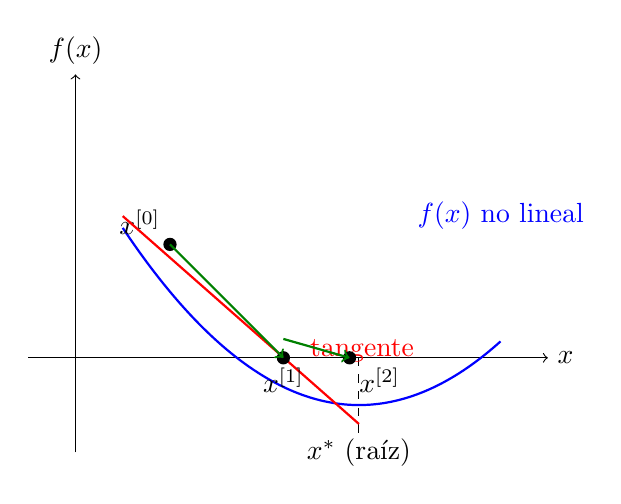
\begin{tikzpicture}[scale=1.2]
% Axes
\draw[->] (-0.5,0) -- (5,0) node[right] {$x$};
\draw[->] (0,-1) -- (0,3) node[above] {$f(x)$};

% Nonlinear function
\draw[thick, blue, domain=0.5:4.5, samples=100] plot (\x, {0.3*(\x-3)^2 - 0.5});
\node[blue] at (4.5, 1.5) {$f(x)$ no lineal};

% Root
\draw[dashed] (3,0) -- (3,-0.8);
\node at (3,-1) {$x^*$ (raíz)};

% First iteration
\coordinate (x0) at (1, 1.2);
\coordinate (x1) at (2.2, 0);

\fill (x0) circle (2pt) node[above left] {$x^{[0]}$};
\draw[red, thick] (0.5, 1.5) -- (3, -0.7) node[near end, above right] {tangente};
\fill (x1) circle (2pt) node[below] {$x^{[1]}$};
\draw[->, thick, green!50!black] (x0) -- (x1);

% Second iteration
\coordinate (x2) at (2.9, 0);
\fill (x2) circle (2pt) node[below right] {$x^{[2]}$};
\draw[->, thick, green!50!black] (2.2, 0.2) -- (x2);

\end{tikzpicture}
\caption{Método de Newton: aproximaciones lineales sucesivas}
\end{figure}

\subsubsection{SQP: Newton Aplicado a Optimización}

SQP hace lo mismo pero con \textbf{aproximaciones cuadráticas} del problema de optimización:

\begin{center}
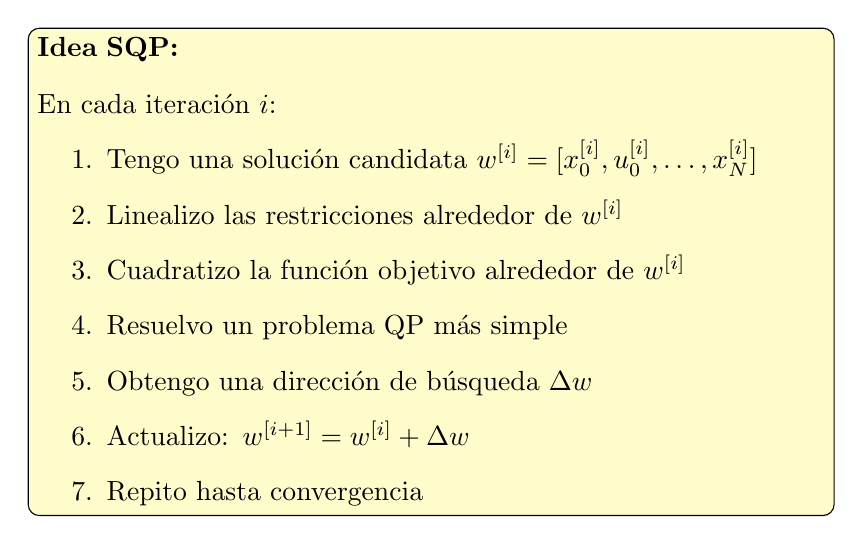
\begin{tikzpicture}
\node[draw, rounded corners, fill=yellow!20, text width=10cm, align=left] {
\textbf{Idea SQP:} \\[0.3cm]
En cada iteración $i$:
\begin{enumerate}
\item Tengo una solución candidata $w^{[i]} = [x_0^{[i]}, u_0^{[i]}, \ldots, x_N^{[i]}]$
\item Linealizo las restricciones alrededor de $w^{[i]}$
\item Cuadratizo la función objetivo alrededor de $w^{[i]}$
\item Resuelvo un problema QP más simple
\item Obtengo una dirección de búsqueda $\Delta w$
\item Actualizo: $w^{[i+1]} = w^{[i]} + \Delta w$
\item Repito hasta convergencia
\end{enumerate}
};
\end{tikzpicture}
\end{center}

\subsection{Paso a Paso: Construyendo el Subproblema QP}

\subsubsection{Paso 1: Definir las Variables de Optimización}

Concatenamos todas las variables de decisión en un vector grande:

\begin{equation}
w = \begin{bmatrix} x_0 \\ u_0 \\ x_1 \\ u_1 \\ \vdots \\ u_{N-1} \\ x_N \end{bmatrix} \in \mathbb{R}^{(N+1)n_x + Nn_u}
\end{equation}

Para tu péndulo invertido con $n_x = 4$, $n_u = 2$, $N = 40$:
\begin{equation}
w \in \mathbb{R}^{41 \times 4 + 40 \times 2} = \mathbb{R}^{244}
\end{equation}

\subsubsection{Paso 2: Linealizar las Restricciones de Dinámica}

La restricción no lineal de dinámica es:

\begin{equation}
h_k(w) := x_{k+1} - \varphi(x_k, u_k) = 0
\end{equation}

En la iteración $i$, tenemos $w^{[i]}$. Aproximamos con Taylor de primer orden:

\begin{align}
h_k(w^{[i]} + \Delta w) &\approx h_k(w^{[i]}) + \frac{\partial h_k}{\partial w}\bigg|_{w^{[i]}} \Delta w \\
&= \underbrace{(x_{k+1}^{[i]} - \varphi(x_k^{[i]}, u_k^{[i]}))}_{\bar{\varphi}_k^x - x_{k+1}^{[i]}} + \begin{bmatrix} -A_k & -B_k & I & 0 & \cdots \end{bmatrix} \Delta w
\end{align}

donde definimos las \textbf{matrices Jacobianas}:

\begin{equation}
\boxed{
A_k := \frac{\partial \varphi}{\partial x}\bigg|_{(x_k^{[i]}, u_k^{[i]})}, \quad
B_k := \frac{\partial \varphi}{\partial u}\bigg|_{(x_k^{[i]}, u_k^{[i]})}
}
\end{equation}

\begin{center}
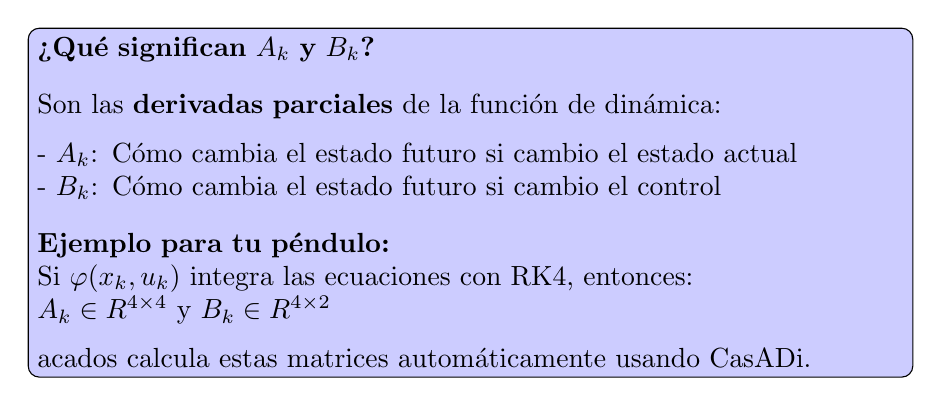
\begin{tikzpicture}
\node[draw, rounded corners, fill=blue!20, text width=11cm, align=left] {
\textbf{¿Qué significan $A_k$ y $B_k$?} \\[0.3cm]
Son las \textbf{derivadas parciales} de la función de dinámica: \\[0.2cm]
- $A_k$: Cómo cambia el estado futuro si cambio el estado actual \\
- $B_k$: Cómo cambia el estado futuro si cambio el control \\[0.3cm]
\textbf{Ejemplo para tu péndulo:} \\
Si $\varphi(x_k, u_k)$ integra las ecuaciones con RK4, entonces: \\
$A_k \in \mathbb{R}^{4 \times 4}$ y $B_k \in \mathbb{R}^{4 \times 2}$ \\[0.2cm]
acados calcula estas matrices automáticamente usando CasADi.
};
\end{tikzpicture}
\end{center}

Reformulando en términos de $\Delta w = w - w^{[i]}$:

\begin{equation}
\Delta x_{k+1} = A_k \Delta x_k + B_k \Delta u_k + \underbrace{(\bar{\varphi}_k^x - x_{k+1}^{[i]})}_{\text{error residual}}
\end{equation}

\subsubsection{Paso 3: Linealizar las Restricciones de Desigualdad}

Para las restricciones de camino $g(x_k, u_k) \leq 0$:

\begin{equation}
g(x_k^{[i]} + \Delta x_k, u_k^{[i]} + \Delta u_k) \approx g(x_k^{[i]}, u_k^{[i]}) + G_k^x \Delta x_k + G_k^u \Delta u_k
\end{equation}

donde:

\begin{equation}
\boxed{
G_k^x := \frac{\partial g}{\partial x}\bigg|_{(x_k^{[i]}, u_k^{[i]})}, \quad
G_k^u := \frac{\partial g}{\partial u}\bigg|_{(x_k^{[i]}, u_k^{[i]})}
}
\end{equation}

Reordenando:

\begin{equation}
G_k^x \Delta x_k + G_k^u \Delta u_k \leq -g(x_k^{[i]}, u_k^{[i]}) =: -\bar{g}_k
\end{equation}

\subsubsection{Paso 4: Cuadratizar la Función Objetivo}

Para el costo, usamos aproximación de Taylor de segundo orden:

\begin{align}
J(w^{[i]} + \Delta w) &\approx J(w^{[i]}) + \nabla J(w^{[i]})^T \Delta w + \frac{1}{2} \Delta w^T H(w^{[i]}) \Delta w
\end{align}

Pero como $J(w^{[i]})$ es constante para la optimización, lo ignoramos:

\begin{equation}
\min_{\Delta w} \quad \underbrace{\nabla J^T \Delta w}_{\text{parte lineal}} + \underbrace{\frac{1}{2} \Delta w^T H \Delta w}_{\text{parte cuadrática}}
\end{equation}

\paragraph{¿Qué es $H$? El Hessiano}

\begin{equation}
H = \nabla^2 J(w^{[i]}) = \begin{bmatrix}
\frac{\partial^2 J}{\partial x_0^2} & \frac{\partial^2 J}{\partial x_0 \partial u_0} & \cdots \\
\vdots & \ddots & \vdots \\
\cdots & \cdots & \frac{\partial^2 J}{\partial x_N^2}
\end{bmatrix}
\end{equation}

\textbf{Problema:} Calcular el Hessiano exacto es muy costoso computacionalmente.

\textbf{Solución en acados:} Usar \textbf{aproximación de Gauss-Newton}.

\subsubsection{Aproximación de Gauss-Newton del Hessiano}

Para un costo de mínimos cuadrados (como el tuyo):

\begin{equation}
\ell(x_k, u_k) = \left\| \begin{bmatrix} x_k \\ u_k \end{bmatrix} \right\|_W^2 = r_k^T W r_k
\end{equation}

donde $r_k = \begin{bmatrix} x_k \\ u_k \end{bmatrix}$.

El Hessiano exacto sería:

\begin{equation}
H_k^{\text{exact}} = \frac{\partial^2 \ell_k}{\partial (x_k, u_k)^2} = 2W + \underbrace{\text{términos de segunda derivada}}_{\text{costosos y pequeños}}
\end{equation}

\textbf{Gauss-Newton ignora los términos de segunda derivada:}

\begin{equation}
\boxed{
H_k^{\text{GN}} = 2 \left(\frac{\partial r_k}{\partial (x_k, u_k)}\right)^T W \left(\frac{\partial r_k}{\partial (x_k, u_k)}\right) = 2 \begin{bmatrix} I \\ I \end{bmatrix}^T W \begin{bmatrix} I \\ I \end{bmatrix} = 2W
}
\end{equation}

Para tu caso específico:

\begin{equation}
H_k = \begin{bmatrix} W_x & 0 \\ 0 & W_u \end{bmatrix} = \begin{bmatrix}
200 & 0 & 0 & 0 & 0 & 0 \\
0 & 2000 & 0 & 0 & 0 & 0 \\
0 & 0 & 200 & 0 & 0 & 0 \\
0 & 0 & 0 & 2000 & 0 & 0 \\
0 & 0 & 0 & 0 & 0.2 & 0 \\
0 & 0 & 0 & 0 & 0 & 0.2
\end{bmatrix}
\end{equation}

\subsection{El Subproblema QP Completo}

Juntando todo, en cada iteración SQP resolvemos:

\begin{equation}
\begin{aligned}
\min_{\Delta x_0, \Delta u_0, \ldots, \Delta x_N} \quad & \sum_{k=0}^{N-1} \left[ \begin{bmatrix} \Delta x_k \\ \Delta u_k \end{bmatrix}^T H_k \begin{bmatrix} \Delta x_k \\ \Delta u_k \end{bmatrix} + \begin{bmatrix} q_k \\ r_k \end{bmatrix}^T \begin{bmatrix} \Delta x_k \\ \Delta u_k \end{bmatrix} \right] \\
& + \Delta x_N^T Q_N \Delta x_N + q_N^T \Delta x_N \\
\text{sujeto a} \quad & \Delta x_0 = 0 \quad \text{(estado inicial fijo)}, \\
& \Delta x_{k+1} = A_k \Delta x_k + B_k \Delta u_k + b_k, \quad k=0,\ldots,N-1, \\
& G_k^x \Delta x_k + G_k^u \Delta u_k \leq d_k, \quad k=0,\ldots,N-1,
\end{aligned}
\end{equation}

donde:
\begin{align}
b_k &= \bar{\varphi}_k^x - x_{k+1}^{[i]} \quad \text{(residuo de dinámica)} \\
d_k &= -\bar{g}_k = -g(x_k^{[i]}, u_k^{[i]}) \quad \text{(residuo de restricciones)} \\
q_k, r_k &= \nabla_{x_k, u_k} \ell(x_k^{[i]}, u_k^{[i]}) \quad \text{(gradiente del costo)}
\end{align}

\begin{center}
\fcolorbox{red}{yellow!20}{
\parbox{0.85\textwidth}{
\textbf{¡Este es un Problema de Programación Cuadrática (QP)!} \\[0.3cm]
- Función objetivo: cuadrática en $\Delta w$ \\
- Restricciones: todas lineales en $\Delta w$ \\
- Los solvers de QP (como HPIPM) pueden resolverlo MUY rápido
}
}
\end{center}

\subsection{Diagrama del Flujo SQP Completo}

\begin{figure}[h]
\centering
\begin{tikzpicture}[node distance=2cm, auto,
    block/.style={rectangle, draw, fill=blue!20, text width=5cm, text centered, rounded corners, minimum height=1.5cm},
    decision/.style={diamond, draw, fill=green!20, text width=3cm, text centered, aspect=2},
    arrow/.style={->, >=stealth, thick}
]

\node[block] (init) {
\textbf{Inicializar} \\
$w^{[0]} = [x_0^{[0]}, u_0^{[0]}, \ldots]$ \\
(guess inicial)
};

\node[block, below=of init] (eval) {
\textbf{Evaluar en $w^{[i]}$:} \\
- $\varphi(x_k^{[i]}, u_k^{[i]})$ (dinámica) \\
- $g(x_k^{[i]}, u_k^{[i]})$ (restricciones) \\
- $\ell(x_k^{[i]}, u_k^{[i]})$ (costo)
};

\node[block, below=of eval] (linearize) {
\textbf{Linealizar/Cuadratizar:} \\
- Calcular $A_k, B_k$ (Jacobianos dinámica) \\
- Calcular $G_k^x, G_k^u$ (Jacobianos restricciones) \\
- Calcular $H_k$ (Hessiano aproximado)
};

\node[block, below=of linearize] (qp) {
\textbf{Resolver QP} \\
Obtener dirección $\Delta w^{[i]}$ \\
(usando HPIPM)
};

\node[block, below=of qp] (update) {
\textbf{Actualizar} \\
$w^{[i+1]} = w^{[i]} + \Delta w^{[i]}$
};

\node[decision, below=of update] (converged) {
¿Convergió? \\
$\|\Delta w\| < \epsilon$
};

\node[block, right=3cm of converged] (done) {
\textbf{Solución óptima} \\
$w^* = w^{[i+1]}$ \\
Aplicar $u_0^*$
};

% Arrows
\draw[arrow] (init) -- (eval);
\draw[arrow] (eval) -- (linearize);
\draw[arrow] (linearize) -- (qp);
\draw[arrow] (qp) -- (update);
\draw[arrow] (update) -- (converged);
\draw[arrow] (converged) -- node[near start] {SÍ} (done);
\draw[arrow] (converged.west) -- node[near start] {NO} ++(-2,0) |- (eval.west);

\node[text width=3cm, align=center] at (-4, -8) {$i = i+1$};

\end{tikzpicture}
\caption{Flujo completo del algoritmo SQP}
\end{figure}

\subsection{Real-Time Iteration (RTI): La Versión Rápida}

En tu código usas \texttt{SQP\_RTI}, que es una versión simplificada para tiempo real:

\begin{center}
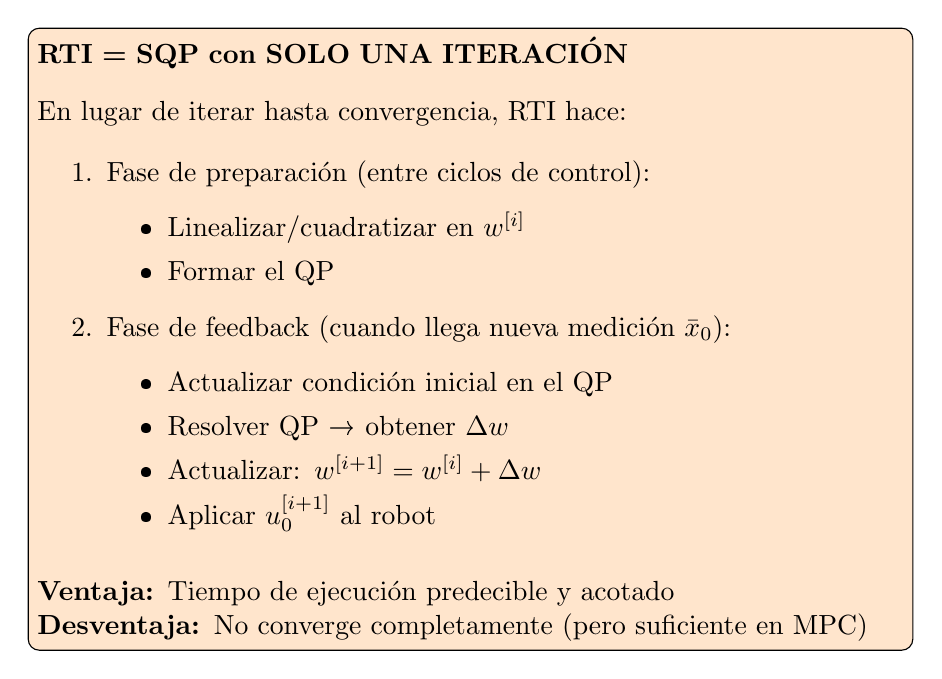
\begin{tikzpicture}
\node[draw, rounded corners, fill=orange!20, text width=11cm, align=left] {
\textbf{RTI = SQP con SOLO UNA ITERACIÓN} \\[0.3cm]
En lugar de iterar hasta convergencia, RTI hace: \\[0.2cm]
\begin{enumerate}
\item Fase de preparación (entre ciclos de control):
    \begin{itemize}
    \item Linealizar/cuadratizar en $w^{[i]}$
    \item Formar el QP
    \end{itemize}
\item Fase de feedback (cuando llega nueva medición $\bar{x}_0$):
    \begin{itemize}
    \item Actualizar condición inicial en el QP
    \item Resolver QP → obtener $\Delta w$
    \item Actualizar: $w^{[i+1]} = w^{[i]} + \Delta w$
    \item Aplicar $u_0^{[i+1]}$ al robot
    \end{itemize}
\end{enumerate}
\vspace{0.2cm}
\textbf{Ventaja:} Tiempo de ejecución predecible y acotado \\
\textbf{Desventaja:} No converge completamente (pero suficiente en MPC)
};
\end{tikzpicture}
\end{center}

\subsection{Ejemplo Numérico Simplificado}

Consideremos un problema super simple para ver los números:

\subsubsection{Sistema}
\begin{equation}
x_{k+1} = x_k + u_k, \quad x_0 = 5
\end{equation}

\subsubsection{Objetivo}
\begin{equation}
\min \sum_{k=0}^{2} (x_k^2 + 0.1 u_k^2) + 10 x_3^2
\end{equation}

\subsubsection{Restricciones}
\begin{equation}
-2 \leq u_k \leq 2
\end{equation}

\paragraph{Iteración SQP 0:}

Guess inicial: $w^{[0]} = [x_0=5, u_0=0, x_1=5, u_1=0, x_2=5, u_2=0, x_3=5]$

\textbf{1. Evaluar:}
\begin{align}
\varphi_0(5, 0) &= 5 + 0 = 5 \\
\ell_0(5, 0) &= 25 + 0 = 25
\end{align}

\textbf{2. Linealizar dinámica:}
\begin{equation}
A_k = \frac{\partial(x_k + u_k)}{\partial x_k} = 1, \quad B_k = \frac{\partial(x_k + u_k)}{\partial u_k} = 1
\end{equation}

Residuo: $b_0 = \varphi_0(x_0^{[0]}, u_0^{[0]}) - x_1^{[0]} = 5 - 5 = 0$

\textbf{3. Cuadratizar costo:}
\begin{equation}
H_0 = \begin{bmatrix} 2 & 0 \\ 0 & 0.2 \end{bmatrix}, \quad \begin{bmatrix} q_0 \\ r_0 \end{bmatrix} = \begin{bmatrix} 2 \cdot 5 \\ 0.2 \cdot 0 \end{bmatrix} = \begin{bmatrix} 10 \\ 0 \end{bmatrix}
\end{equation}

\textbf{4. Resolver QP:}
\begin{equation}
\begin{aligned}
\min_{\Delta u_0, \Delta u_1, \Delta u_2} \quad & 25 + 10\Delta u_0 + 0.1\Delta u_0^2 + \cdots \\
\text{s.a.} \quad & \Delta x_1 = \Delta x_0 + \Delta u_0 \\
& -2 \leq \Delta u_k + u_k^{[0]} \leq 2
\end{aligned}
\end{equation}

Solución del QP: $\Delta u_0 = -2, \Delta u_1 = -1.5, \Delta u_2 = -1.1$

\textbf{5. Actualizar:}
\begin{equation}
w^{[1]} = w^{[0]} + \Delta w = [5, -2, 3, -1.5, 1.5, -1.1, 0.4]
\end{equation}

¡Y repetimos!


